%\sse{Stabilité de la décomposition lorsque l'on tend vers une application affine}

%La décomposition géométrique ne s'applique pas dans le cas des applications affines,  on doit utiliser la méthode multi-étapes. L'expérience suivante montre la continuité de la méthode lorsque l'on considère une suite d'homographies qui converge ponctuellement vers une affinité (cf figure \ref{image_converge_building}). Il n'y a pas de flou ou d'\emph{aliasing} notable juste avant de passer à une affinité, ni de différence visuelle.

%\begin{figure}[h!]
%		\centering
%		\subfigure{
%		{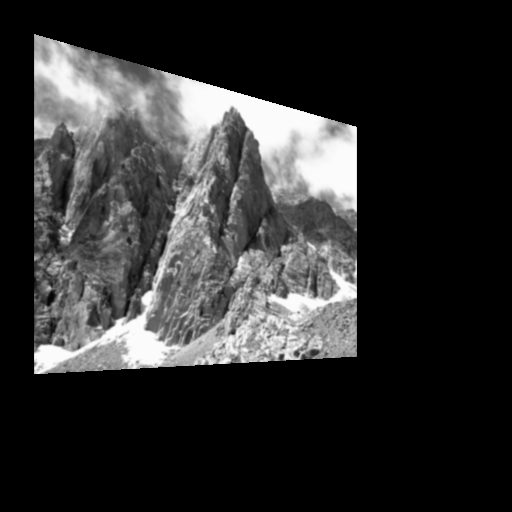
\includegraphics[width=40mm]{test_homo_conv1.png}}
%		{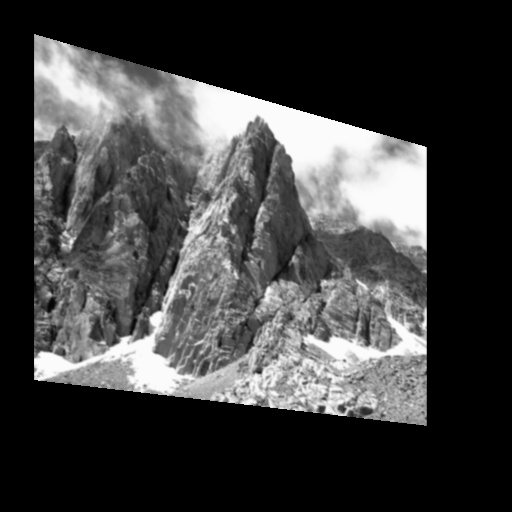
\includegraphics[width=40mm]{test_homo_conv3.png}}
%	    {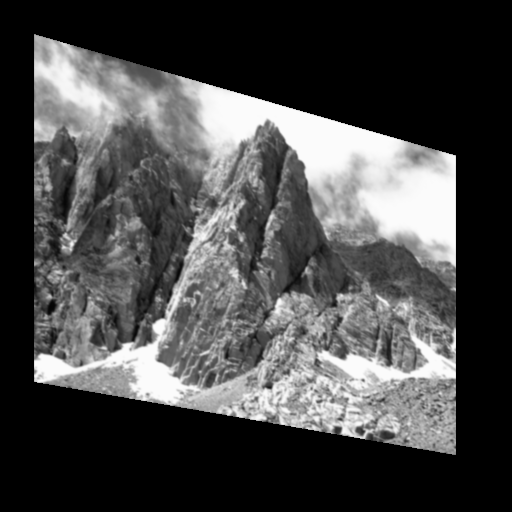
\includegraphics[width=40mm]{test_homo_conv4.png}}}
%		\subfigure{
%		{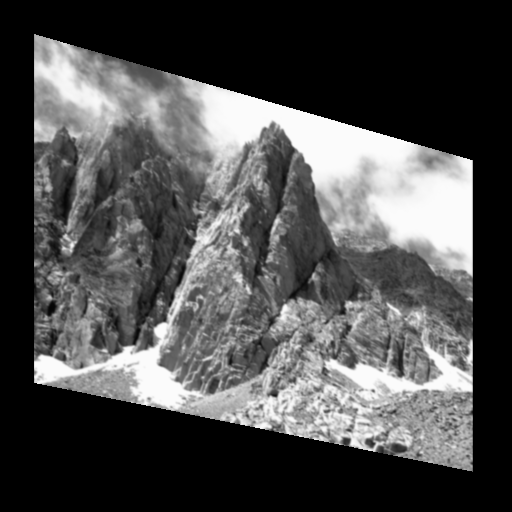
\includegraphics[width=40mm]{test_homo_conv5.png}}
%		{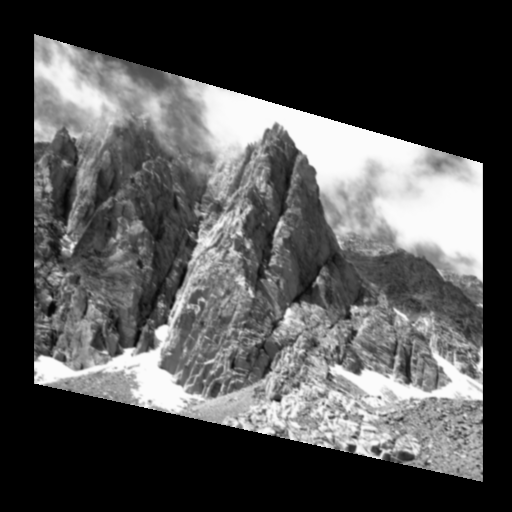
\includegraphics[width=40mm]{test_homo_conv6.png}}
%		{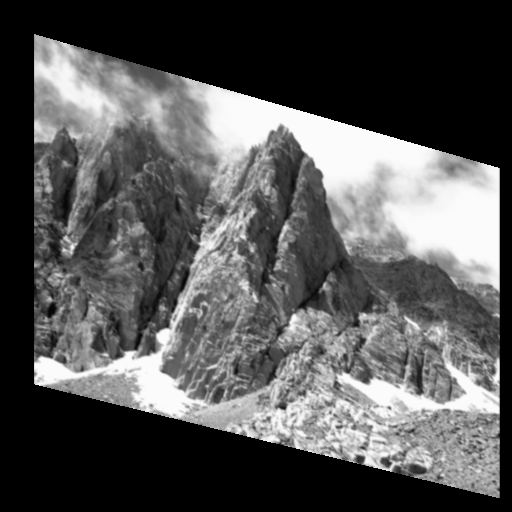
\includegraphics[width=40mm]{test_homo_conv9.png}}}\\
%		\caption{Convergence vers une application affine la dernière image est la limite}
%\label{image_converge_building}
%\end{figure}

\subsection{Continuity of the decomposition when appoaching an affinity}

The geometric decomposition can not resample an affinity (which is a limit case), the multi-pass resampling must be used. The following experiment shows the continuity of the geometric method when a homography sequence tends pointwise to an affinity (cf. figure \ref{image_converge_building}). The is no notable blurring neither aliasing just before the affinity, nor visual difference.

\begin{figure}[h!]
	\centering
	\subfigure{
	{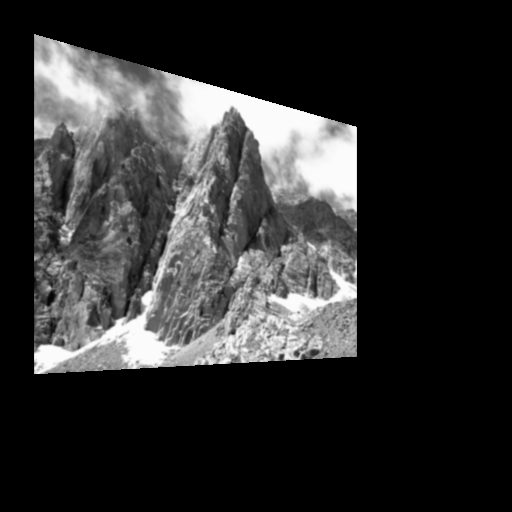
\includegraphics[width=40mm]{test_homo_conv1.png}}
	{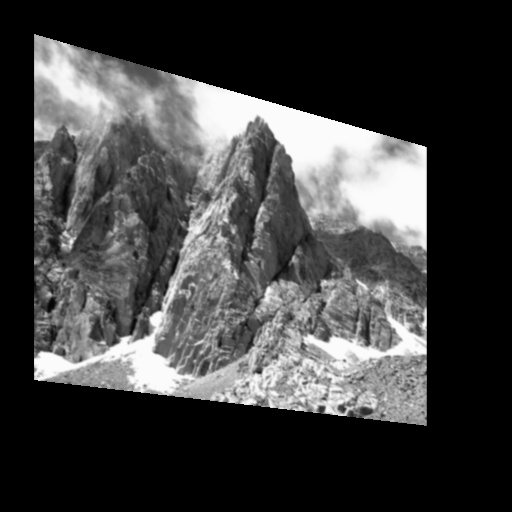
\includegraphics[width=40mm]{test_homo_conv3.png}}
	{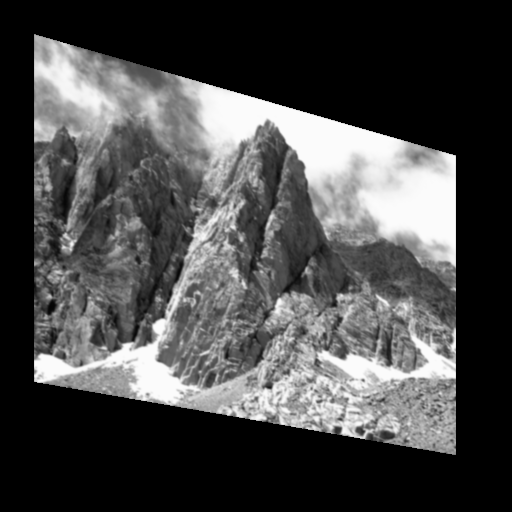
\includegraphics[width=40mm]{test_homo_conv4.png}}}
	\subfigure{
	{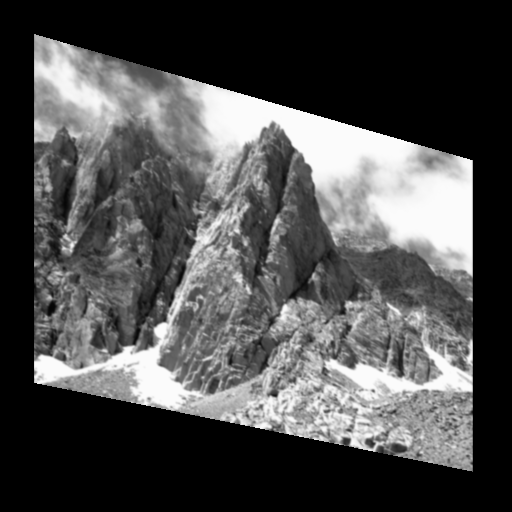
\includegraphics[width=40mm]{test_homo_conv5.png}}
	{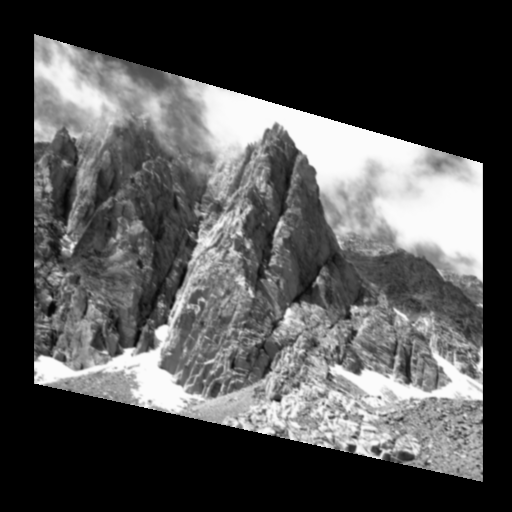
\includegraphics[width=40mm]{test_homo_conv6.png}}
	{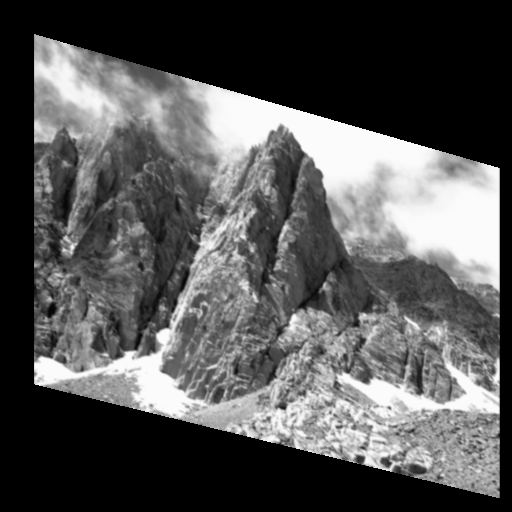
\includegraphics[width=40mm]{test_homo_conv9.png}}}\\
	\caption{Convergence to an affinity ; the last image represent the affinity}
	\label{image_converge_building}
\end{figure}
